% Options for packages loaded elsewhere
\PassOptionsToPackage{unicode,linktoc=all,pdfwindowui,pdfpagemode=FullScreen}{hyperref}
\PassOptionsToPackage{hyphens}{url}
\PassOptionsToPackage{dvipsnames,svgnames,x11names}{xcolor}
%
\documentclass[
  letterpaper,
  DIV=11,
  numbers=noendperiod]{scrreprt}

\usepackage{amsmath,amssymb}
\usepackage{iftex}
\ifPDFTeX
  \usepackage[T1]{fontenc}
  \usepackage[utf8]{inputenc}
  \usepackage{textcomp} % provide euro and other symbols
\else % if luatex or xetex
  \usepackage{unicode-math}
  \defaultfontfeatures{Scale=MatchLowercase}
  \defaultfontfeatures[\rmfamily]{Ligatures=TeX,Scale=1}
\fi
\usepackage{lmodern}
\ifPDFTeX\else  
    % xetex/luatex font selection
\fi
% Use upquote if available, for straight quotes in verbatim environments
\IfFileExists{upquote.sty}{\usepackage{upquote}}{}
\IfFileExists{microtype.sty}{% use microtype if available
  \usepackage[]{microtype}
  \UseMicrotypeSet[protrusion]{basicmath} % disable protrusion for tt fonts
}{}
\usepackage{xcolor}
\setlength{\emergencystretch}{3em} % prevent overfull lines
\setcounter{secnumdepth}{5}
% Make \paragraph and \subparagraph free-standing
\makeatletter
\ifx\paragraph\undefined\else
  \let\oldparagraph\paragraph
  \renewcommand{\paragraph}{
    \@ifstar
      \xxxParagraphStar
      \xxxParagraphNoStar
  }
  \newcommand{\xxxParagraphStar}[1]{\oldparagraph*{#1}\mbox{}}
  \newcommand{\xxxParagraphNoStar}[1]{\oldparagraph{#1}\mbox{}}
\fi
\ifx\subparagraph\undefined\else
  \let\oldsubparagraph\subparagraph
  \renewcommand{\subparagraph}{
    \@ifstar
      \xxxSubParagraphStar
      \xxxSubParagraphNoStar
  }
  \newcommand{\xxxSubParagraphStar}[1]{\oldsubparagraph*{#1}\mbox{}}
  \newcommand{\xxxSubParagraphNoStar}[1]{\oldsubparagraph{#1}\mbox{}}
\fi
\makeatother

\usepackage{color}
\usepackage{fancyvrb}
\newcommand{\VerbBar}{|}
\newcommand{\VERB}{\Verb[commandchars=\\\{\}]}
\DefineVerbatimEnvironment{Highlighting}{Verbatim}{commandchars=\\\{\}}
% Add ',fontsize=\small' for more characters per line
\usepackage{framed}
\definecolor{shadecolor}{RGB}{241,243,245}
\newenvironment{Shaded}{\begin{snugshade}}{\end{snugshade}}
\newcommand{\AlertTok}[1]{\textcolor[rgb]{0.68,0.00,0.00}{#1}}
\newcommand{\AnnotationTok}[1]{\textcolor[rgb]{0.37,0.37,0.37}{#1}}
\newcommand{\AttributeTok}[1]{\textcolor[rgb]{0.40,0.45,0.13}{#1}}
\newcommand{\BaseNTok}[1]{\textcolor[rgb]{0.68,0.00,0.00}{#1}}
\newcommand{\BuiltInTok}[1]{\textcolor[rgb]{0.00,0.23,0.31}{#1}}
\newcommand{\CharTok}[1]{\textcolor[rgb]{0.13,0.47,0.30}{#1}}
\newcommand{\CommentTok}[1]{\textcolor[rgb]{0.37,0.37,0.37}{#1}}
\newcommand{\CommentVarTok}[1]{\textcolor[rgb]{0.37,0.37,0.37}{\textit{#1}}}
\newcommand{\ConstantTok}[1]{\textcolor[rgb]{0.56,0.35,0.01}{#1}}
\newcommand{\ControlFlowTok}[1]{\textcolor[rgb]{0.00,0.23,0.31}{\textbf{#1}}}
\newcommand{\DataTypeTok}[1]{\textcolor[rgb]{0.68,0.00,0.00}{#1}}
\newcommand{\DecValTok}[1]{\textcolor[rgb]{0.68,0.00,0.00}{#1}}
\newcommand{\DocumentationTok}[1]{\textcolor[rgb]{0.37,0.37,0.37}{\textit{#1}}}
\newcommand{\ErrorTok}[1]{\textcolor[rgb]{0.68,0.00,0.00}{#1}}
\newcommand{\ExtensionTok}[1]{\textcolor[rgb]{0.00,0.23,0.31}{#1}}
\newcommand{\FloatTok}[1]{\textcolor[rgb]{0.68,0.00,0.00}{#1}}
\newcommand{\FunctionTok}[1]{\textcolor[rgb]{0.28,0.35,0.67}{#1}}
\newcommand{\ImportTok}[1]{\textcolor[rgb]{0.00,0.46,0.62}{#1}}
\newcommand{\InformationTok}[1]{\textcolor[rgb]{0.37,0.37,0.37}{#1}}
\newcommand{\KeywordTok}[1]{\textcolor[rgb]{0.00,0.23,0.31}{\textbf{#1}}}
\newcommand{\NormalTok}[1]{\textcolor[rgb]{0.00,0.23,0.31}{#1}}
\newcommand{\OperatorTok}[1]{\textcolor[rgb]{0.37,0.37,0.37}{#1}}
\newcommand{\OtherTok}[1]{\textcolor[rgb]{0.00,0.23,0.31}{#1}}
\newcommand{\PreprocessorTok}[1]{\textcolor[rgb]{0.68,0.00,0.00}{#1}}
\newcommand{\RegionMarkerTok}[1]{\textcolor[rgb]{0.00,0.23,0.31}{#1}}
\newcommand{\SpecialCharTok}[1]{\textcolor[rgb]{0.37,0.37,0.37}{#1}}
\newcommand{\SpecialStringTok}[1]{\textcolor[rgb]{0.13,0.47,0.30}{#1}}
\newcommand{\StringTok}[1]{\textcolor[rgb]{0.13,0.47,0.30}{#1}}
\newcommand{\VariableTok}[1]{\textcolor[rgb]{0.07,0.07,0.07}{#1}}
\newcommand{\VerbatimStringTok}[1]{\textcolor[rgb]{0.13,0.47,0.30}{#1}}
\newcommand{\WarningTok}[1]{\textcolor[rgb]{0.37,0.37,0.37}{\textit{#1}}}

\providecommand{\tightlist}{%
  \setlength{\itemsep}{0pt}\setlength{\parskip}{0pt}}\usepackage{longtable,booktabs,array}
\usepackage{calc} % for calculating minipage widths
% Correct order of tables after \paragraph or \subparagraph
\usepackage{etoolbox}
\makeatletter
\patchcmd\longtable{\par}{\if@noskipsec\mbox{}\fi\par}{}{}
\makeatother
% Allow footnotes in longtable head/foot
\IfFileExists{footnotehyper.sty}{\usepackage{footnotehyper}}{\usepackage{footnote}}
\makesavenoteenv{longtable}
\usepackage{graphicx}
\makeatletter
\def\maxwidth{\ifdim\Gin@nat@width>\linewidth\linewidth\else\Gin@nat@width\fi}
\def\maxheight{\ifdim\Gin@nat@height>\textheight\textheight\else\Gin@nat@height\fi}
\makeatother
% Scale images if necessary, so that they will not overflow the page
% margins by default, and it is still possible to overwrite the defaults
% using explicit options in \includegraphics[width, height, ...]{}
\setkeys{Gin}{width=\maxwidth,height=\maxheight,keepaspectratio}
% Set default figure placement to htbp
\makeatletter
\def\fps@figure{htbp}
\makeatother
% definitions for citeproc citations
\NewDocumentCommand\citeproctext{}{}
\NewDocumentCommand\citeproc{mm}{%
  \begingroup\def\citeproctext{#2}\cite{#1}\endgroup}
\makeatletter
 % allow citations to break across lines
 \let\@cite@ofmt\@firstofone
 % avoid brackets around text for \cite:
 \def\@biblabel#1{}
 \def\@cite#1#2{{#1\if@tempswa , #2\fi}}
\makeatother
\newlength{\cslhangindent}
\setlength{\cslhangindent}{1.5em}
\newlength{\csllabelwidth}
\setlength{\csllabelwidth}{3em}
\newenvironment{CSLReferences}[2] % #1 hanging-indent, #2 entry-spacing
 {\begin{list}{}{%
  \setlength{\itemindent}{0pt}
  \setlength{\leftmargin}{0pt}
  \setlength{\parsep}{0pt}
  % turn on hanging indent if param 1 is 1
  \ifodd #1
   \setlength{\leftmargin}{\cslhangindent}
   \setlength{\itemindent}{-1\cslhangindent}
  \fi
  % set entry spacing
  \setlength{\itemsep}{#2\baselineskip}}}
 {\end{list}}
\usepackage{calc}
\newcommand{\CSLBlock}[1]{\hfill\break\parbox[t]{\linewidth}{\strut\ignorespaces#1\strut}}
\newcommand{\CSLLeftMargin}[1]{\parbox[t]{\csllabelwidth}{\strut#1\strut}}
\newcommand{\CSLRightInline}[1]{\parbox[t]{\linewidth - \csllabelwidth}{\strut#1\strut}}
\newcommand{\CSLIndent}[1]{\hspace{\cslhangindent}#1}

::: {.hidden}
\DeclareMathOperator{\EX}{\mathbb{E}}
:::
\KOMAoption{captions}{tableheading}
\usepackage{indentfirst}
\setlength{\parindent}{1.3cm}
\setlength{\parskip}{0.2cm}
\makeatletter
\@ifpackageloaded{bookmark}{}{\usepackage{bookmark}}
\makeatother
\makeatletter
\@ifpackageloaded{caption}{}{\usepackage{caption}}
\AtBeginDocument{%
\ifdefined\contentsname
  \renewcommand*\contentsname{Índice}
\else
  \newcommand\contentsname{Índice}
\fi
\ifdefined\listfigurename
  \renewcommand*\listfigurename{Lista de Figuras}
\else
  \newcommand\listfigurename{Lista de Figuras}
\fi
\ifdefined\listtablename
  \renewcommand*\listtablename{Lista de Tabelas}
\else
  \newcommand\listtablename{Lista de Tabelas}
\fi
\ifdefined\figurename
  \renewcommand*\figurename{Figura}
\else
  \newcommand\figurename{Figura}
\fi
\ifdefined\tablename
  \renewcommand*\tablename{Tabela}
\else
  \newcommand\tablename{Tabela}
\fi
}
\@ifpackageloaded{float}{}{\usepackage{float}}
\floatstyle{ruled}
\@ifundefined{c@chapter}{\newfloat{codelisting}{h}{lop}}{\newfloat{codelisting}{h}{lop}[chapter]}
\floatname{codelisting}{Listagem}
\newcommand*\listoflistings{\listof{codelisting}{Lista de Listagens}}
\usepackage{amsthm}
\theoremstyle{definition}
\newtheorem{definition}{Definição}[chapter]
\theoremstyle{plain}
\newtheorem{theorem}{Teorema}[chapter]
\theoremstyle{remark}
\AtBeginDocument{\renewcommand*{\proofname}{Comprovação}}
\newtheorem*{remark}{Comentário}
\newtheorem*{solution}{Solução}
\newtheorem{refremark}{Comentário}[chapter]
\newtheorem{refsolution}{Solução}[chapter]
\makeatother
\makeatletter
\makeatother
\makeatletter
\@ifpackageloaded{caption}{}{\usepackage{caption}}
\@ifpackageloaded{subcaption}{}{\usepackage{subcaption}}
\makeatother

\ifLuaTeX
\usepackage[bidi=basic]{babel}
\else
\usepackage[bidi=default]{babel}
\fi
\babelprovide[main,import]{portuguese}
% get rid of language-specific shorthands (see #6817):
\let\LanguageShortHands\languageshorthands
\def\languageshorthands#1{}
\ifLuaTeX
  \usepackage{selnolig}  % disable illegal ligatures
\fi
\usepackage{bookmark}

\IfFileExists{xurl.sty}{\usepackage{xurl}}{} % add URL line breaks if available
\urlstyle{same} % disable monospaced font for URLs
\hypersetup{
  pdftitle={Notas em Econometria},
  pdfauthor={Gabriel Arruda},
  pdflang={pt},
  colorlinks=true,
  linkcolor={blue},
  filecolor={Maroon},
  citecolor={Blue},
  urlcolor={Blue},
  pdfcreator={LaTeX via pandoc}}


\title{Notas em Econometria}
\usepackage{etoolbox}
\makeatletter
\providecommand{\subtitle}[1]{% add subtitle to \maketitle
  \apptocmd{\@title}{\par {\large #1 \par}}{}{}
}
\makeatother
\subtitle{Teoria e Aplicação}
\author{Gabriel Arruda}
\date{2024-08-01}

\begin{document}
\maketitle

\renewcommand*\contentsname{Índice}
{
\hypersetup{linkcolor=}
\setcounter{tocdepth}{2}
\tableofcontents
}

\bookmarksetup{startatroot}

\chapter*{Disclaimer}\label{disclaimer}
\addcontentsline{toc}{chapter}{Disclaimer}

\markboth{Disclaimer}{Disclaimer}

Este projeto teve início com base nas notas de aula do
Prof.~Dr.~Fernando Aiube e do Prof.~Dr.~Francis Petterini, assim como
nas notas de aula do Kotze (2019) e nos livros: Box et al. (2015),
Hamilton (1994) e Enders (2014). O trabalho ainda precisa ser concluído
e revisado. Vale destacar que pretendo incluir formas de aplicar os
modelos em \textit{Python}.

A idealização do projeto surgiu como uma maneira de estudo para eu
aprender tanto a teoria quanto a aplicação prática de cada modelo. A
implementação dos modelos será feita do zero, utilizando o mínimo de
pacotes possível.

Alguns scripts estarão disponíveis dentro do texto, mas todos poderão
ser acessados no meu \href{https://github.com/g-arruda}{GitHub}.

Lembrando que a ideia é sempre utilizar o minimo de pacotes possiveis:

\begin{Shaded}
\begin{Highlighting}[]
\CommentTok{\# Importações globais}
\ImportTok{import}\NormalTok{ pandas }\ImportTok{as}\NormalTok{ pd}
\ImportTok{import}\NormalTok{ numpy }\ImportTok{as}\NormalTok{ np}
\ImportTok{import}\NormalTok{ matplotlib.pyplot }\ImportTok{as}\NormalTok{ plt}
\end{Highlighting}
\end{Shaded}

\bookmarksetup{startatroot}

\chapter{Introdução}\label{introduuxe7uxe3o}

\section{Regressão linear}\label{regressuxe3o-linear}

Regressão linear é uma ferramenta estatística usada para modelar a
relação entre uma variável dependente e uma ou mais variáveis
independentes, assumindo que essa relação pode ser descrita por uma
linha reta. A ideia de se utilizar é uma é dado a sua simplicidade,
tendo apenas um parâmetro de inclinação e um de intercepto, uma outra é
que aqui se assume que as variáveis apresentam uma relação linear. A
linha representa a melhor aproximação da tendência central dos dados.
Aqui devemos partir de uma amostra, um par ordenado
\(\{x_{i},y_{i}\}^{N}_{i=1}\), encontrar uma reta que melhor se ajusta a
média dos dados, para isso, vamos partir da equação de uma reta. \[
y=\alpha + \beta x
\]

Onde a ideia aqui é querer entender qual relação em que a variável \(x\)
afeta a variável \(y\), temos então que resolver dois problemas:
primeiro é encontrar os parâmetros \(\alpha\) e \(\beta\) que melhor se
ajusta, sabendo que nem todo o \(y\) pode ser explicado pelo \(x\),
temos que adicionar uma variável à equação que consiga captar essa
relação no modelo, essa variável será dada por \(u\).

Podemos reescrever a equação acima como sendo um sistema de equações
lineares \[
\begin{aligned}
  y_{1} &= \alpha + \beta x_{1} + u_{1} \\
  y_{2} &= \alpha + \beta x_{2} + u_{2} \\
  y_{3} &= \alpha + \beta x_{3} + u_{3} \\
  & \vdots \\
  y_{n} &= \alpha + \beta x_{n} + u_{n}
\end{aligned}
\]

Note que esse é um sistema de \(n\) equações lineares com \(n + 2\)
incógnitas. E que pela regra de Cramer, sabemos que o sistema apresenta
infinitas soluções. O que não nos ajuda e precisamos voltar ao problema,
quais valores de \(\alpha\) e \(\beta\) que melhor se ajusta? Uma
maneira de se fazer isso, é minimizar a soma do erro quadrático
\(\left(\sum_{i=1}^{N} u_i^{2}\right)\) e para isso, vamos isolar o
erro, elevar tudo ao quadrado e aplicar a recursividade. \[
\sum_{i=1}^{N} u_i^{2} = \sum_{i=1}^{N} (y_{i} - \alpha - \beta x_{i})^{2}
\]

Dado isso, podemos dizer que podemos estimar valores de \(\alpha\) e
\(\beta\) que minimizam o erro quadrático. Seja
\(S(\alpha, \beta) = \sum_{i=1}^{N} u_i^{2}\) e sabendo que os valores
dos parâmetros que zeram o gradiente
\(\nabla = \left(\frac{\partial S}{\partial \hat{\alpha}}, \frac{\partial S}{\partial \hat{\beta}}\right)=0\)
são os valores que minimizam o erro quadrático. Fazendo as
derivadas\ldots{} \[
\begin{aligned}
  \nabla = \begin{bmatrix}
    \dfrac{\partial S}{\partial \hat{\alpha}} \\
    \dfrac{\partial S}{\partial \hat{\beta}}
  \end{bmatrix} = \begin{bmatrix}
    -2\sum_{i=1}^{N} (y_{i} - \hat{\alpha} - \hat{\beta} x_{i}) \\
    -2\sum_{i=1}^{N} (y_{i} - \hat{\alpha} - \hat{\beta} x_{i})(x_{i})
  \end{bmatrix} = 0
\end{aligned}
\]

Podemos multiplicar ambos os lados por \(-\frac{1}{2}\) e abrir o
somatório\footnote{Note que se somarmos n vezes um parâmetro é o mesmo
  que dizer n vezes o parâmetro, logo
  \(\sum_{i=1}^{N}\hat{\alpha} = n\hat{\alpha}\).}. \[
\begin{aligned}
  \begin{bmatrix}
    \sum_{i=1}^{N} y_{i} - n\hat{\alpha} - \hat{\beta}\sum_{i=1}^{N} x_{i} \\
    \sum_{i=1}^{N} y_{i}x_{i} - \hat{\alpha}\sum_{i=1}^{N}x_{i} - \hat{\beta}\sum_{i=1}^{N} x_{i}^{2}
  \end{bmatrix} = 0
\end{aligned}
\]

Separando os termos, temos que \[
\begin{aligned}
  \begin{bmatrix}
    \sum_{i=1}^{N} y_{i} \\
    \sum_{i=1}^{N} y_{i}x_{i}
  \end{bmatrix} =
  \begin{bmatrix}
    n\hat{\alpha} + \hat{\beta}\sum_{i=1}^{N} x_{i} \\
    \hat{\alpha}\sum_{i=1}^{N}x_{i} + \hat{\beta}\sum_{i=1}^{N} x_{i}^{2}
  \end{bmatrix}
\end{aligned}
\] \[
\begin{aligned}
  \begin{bmatrix}
    \sum_{i=1}^{N} y_{i} \\
    \sum_{i=1}^{N} y_{i}x_{i}
  \end{bmatrix} =
  \begin{bmatrix}
    n & \sum_{i=1}^{N} x_{i} \\
    \sum_{i=1}^{N} x_{i} & \sum_{i=1}^{N} x_{i}^{2}
  \end{bmatrix}
  \begin{bmatrix}
    \hat{\alpha} \\
    \hat{\beta}
  \end{bmatrix}
\end{aligned}
\]

Podemos reorganizar da seguinte maneira: \[
\begin{bmatrix}
n & \sum_{i=1}^{N} x_{i} \\
\sum_{i=1}^{N} x_{i} & \sum_{i=1}^{N} x_{i}^{2}
\end{bmatrix}
\begin{bmatrix}
\hat{\alpha} \\
\hat{\beta}
\end{bmatrix}
=
\begin{bmatrix}
\sum_{i=1}^{N} y_{i} \\
\sum_{i=1}^{N} y_{i}x_{i}
\end{bmatrix}
\]

Pré-multiplicando ambos os lados pelo inverso da matriz que tem os
valores de \(x\): \[
\begin{bmatrix}
\hat{\alpha} \\
\hat{\beta}
\end{bmatrix}
=
\begin{bmatrix}
n & \sum_{i=1}^{N} x_{i} \\
\sum_{i=1}^{N} x_{i} & \sum_{i=1}^{N} x_{i}^{2}
\end{bmatrix}^{-1}
\begin{bmatrix}
\sum_{i=1}^{N} y_{i} \\
\sum_{i=1}^{N} y_{i}x_{i}
\end{bmatrix}
\]

Para termos certeza de que este é o ponto mínimo, devemos avaliar a
matriz hessiana: \[
H =
\begin{bmatrix}
\dfrac{\partial^2 S}{\partial \alpha^2} & \dfrac{\partial^2 S}{\partial \alpha \, \partial \beta} \\
\dfrac{\partial^2 S}{\partial \alpha \, \partial \beta} & \dfrac{\partial^2 S}{\partial \beta^2}
\end{bmatrix}
\]

Logo: \[
H =
\begin{bmatrix}
n & \sum x_{i} \\
\sum x_{i} & \sum x_{i}^{2}
\end{bmatrix}
\]

Para ser um mínimo global, devemos ter que:

\begin{itemize}
\tightlist
\item
  O primeiro menor principal será \(> 0\)
\item
  O determinante do segundo menor principal será \(>0\)
\end{itemize}

Com isso, podemos dizer que é um ponto de mínimo.

Podemos reescrever: \[
\begin{bmatrix}
n & \sum x_{i} \\
\sum x_{i} & \sum x_{i}^{2}
\end{bmatrix}
\begin{bmatrix}
\hat{\alpha} \\
\hat{\beta}
\end{bmatrix}
=
\begin{bmatrix}
\sum y_{i} \\
\sum x_{i} y_{i}
\end{bmatrix}
\]

Abrindo: \[
\begin{bmatrix}
1 & 1 & \dots & 1 \\
x_{1} & x_{2} & \dots & x_{n}
\end{bmatrix}'
\begin{bmatrix}
1 & x_{1} \\
1 & x_{2} \\
\vdots \\
1 & x_{n}
\end{bmatrix}
\begin{bmatrix}
\hat{\alpha} \\
\hat{\beta}
\end{bmatrix}
=
\begin{bmatrix}
y_{1} \\
y_{2} \\
\vdots \\
y_{n}
\end{bmatrix}
\]

Onde: \[
X =
\begin{bmatrix}
1 & 1 & \dots & 1 \\
x_{1} & x_{2} & \dots & x_{n}
\end{bmatrix}'
\] \[
\hat{B} =
\begin{bmatrix}
\hat{\alpha} \\
\hat{\beta}
\end{bmatrix}
\] \[
Y =
\begin{bmatrix}
y_{1} \\
y_{2} \\
\vdots \\
y_{n}
\end{bmatrix}
\]

Então: \[
X' \hat{B} = X' Y
\] \[
(X' X) \hat{B} = X' Y
\] \[
(X' X)^{-1} (X' X) \hat{B} = (X' X)^{-1} X' Y
\] \[
\hat{B} = (X' X)^{-1} X' Y
\] \[
\boxed{\hat{B} = (X' X)^{-1} X' Y}
\]

Então, sempre que estamos falando do estimador do \textbf{MQO}, estamos
nos referindo à fórmula fechada: \[
\hat{B} = (X' X)^{-1} X' Y
\]

Agora, temos que pensar da seguinte maneira: dado que conseguimos
construir os estimadores, como podemos criar seus intervalos de
confiança? Para isso, podemos substituir \(Y\) por
\(XB + U\):\footnote{Vale lembrar que \(B\) sem chapéu é o melhor ajuste
  possível da reta, os valores que só Deus sabe.} \[
\hat{B} = (X' X)^{-1} X' (XB + U)
\] \[
= (X' X)^{-1} X' XB + (X' X)^{-1} X' U
\]

Assumindo que os dados não tenham problema de multicolinearidade
perfeita, a matriz \((X' X)^{-1}\) deve existir para que
\(I = (X' X)^{-1} X' X\):
\begin{equation}\phantomsection\label{eq-endo}{
\hat{B} = B + (X' X)^{-1} X' U
}\end{equation}

Observamos na equação Equação~\ref{eq-endo} que a componente do
estimador influenciada pelo erro, especificamente \(X' U\), ilustra uma
premissa importante do modelo: \(\mathbb{E}(X | U) = 0\). Isso implica
que, idealmente, todas as variáveis explicativas deveriam ser exógenas,
não apresentando qualquer correlação com o termo de erro. Mas, é
importante reconhecer que, na prática, alcançar uma exogeneidade
completa é praticamente inviável; assim, é realista esperar que qualquer
modelo econômico possa manifestar algum nível, mesmo que mínimo, de
endogeneidade.

Subtraind os dois lados da Equação~\ref{eq-endo} por \(-B\) e
pós-multiplicando por \((\hat{B} - B)'\): \[
(\hat{B} - B)(\hat{B} - B)' = (X' X)^{-1} X' U[(X' X)^{-1} X' U]'
\]

Desenvolvendo a parte esquerda dessa igualdade, temos que: \[
\begin{bmatrix}
\hat{B}_{1} - B \\
\hat{B}_{2} - B
\end{bmatrix}
\begin{bmatrix}
\hat{B}_{1} - B & \hat{B}_{2} - B
\end{bmatrix}'
\]

Multiplicando e aplicando o operador da esperança: \[
\begin{bmatrix}
\mathbb{E}[(\hat{B}_{1} - B)^{2}] & \mathbb{E}[(\hat{B}_{1} - B)(\hat{B}_{2} - B)] \\
\mathbb{E}[(\hat{B}_{1} - B)(\hat{B}_{2} - B)] & \mathbb{E}[(\hat{B}_{2} - B)^{2}]
\end{bmatrix}
\]

Onde a diagonal principal é a variância de \(\hat{B}_{1}\) e o resto é a
covariância, então montamos a matriz de variância-covariância: \[
\begin{bmatrix}
\text{Var}(\hat{B}_{1}) & \text{Cov}(\hat{B}_{1}, \hat{B}_{2}) \\
\text{Cov}(\hat{B}_{1}, \hat{B}_{2}) & \text{Var}(\hat{B}_{2})
\end{bmatrix}
\]

A partir disso, poderíamos montar um intervalo de confiança para os
betas se não fosse um pequeno problema\ldots{} Aqui precisamos do valor
de \(\beta\), e que só Deus sabe. Vamos então olhar para o lado direito
da igualdade\footnote{Vale lembrar que \((AB)' = B' A'\)} \[
=(X' X)^{-1} X' UU' X[(X' X)^{-1}]'
\] \[
=(X' X)^{-1} X' UU' X(X' X)^{-1}
\]

Abrindo \(UU'\) e aplicando o operador da esperança: \[
UU' =
\begin{bmatrix}
u_1 \\
u_2 \\
\vdots \\
u_n
\end{bmatrix}
\begin{bmatrix}
u_1 & u_2 & \cdots & u_n
\end{bmatrix}'
\] \[
=
\begin{bmatrix}
\mathbb{E}(u_1)^{2} & \mathbb{E}(u_1, u_2) & \cdots & \mathbb{E}(u_1, u_n) \\
\mathbb{E}(u_2, u_1) & \mathbb{E}(u_2)^{2} & \cdots & \mathbb{E}(u_2, u_n) \\
\vdots & \vdots & \ddots & \vdots \\
\mathbb{E}(u_n, u_1) & \mathbb{E}(u_n, u_2) & \cdots & \mathbb{E}(u_n)^{2}
\end{bmatrix}
\] Vamos ter que na diagonal principal é a variância dos erros e
\(\forall \, \mathbb{E}(u_{i}, u_{j})\) em que \(i \neq j\) temos a
covariância dos erros. Sob as hipóteses de homoscedasticidade\footnote{Variância
  dos erros é constante, isto é,
  \(\mathbb{E}(u_i^2) = \sigma^2, \, \forall i=1, \ldots, n\)} e não
autocorrelação, vamos ter que:

\[
UU' = \begin{bmatrix}
\sigma^{2} & 0 & \cdots & 0 \\
0 & \sigma^{2} & \cdots & 0 \\
\vdots & \vdots & \ddots & \vdots \\
0 & 0 & \cdots & \sigma^{2}
\end{bmatrix}
\]

\[
= \sigma^{2} \begin{bmatrix}
1 & 0 & \cdots & 0 \\
0 & 1 & \cdots & 0 \\
\vdots & \vdots & \ddots & \vdots \\
0 & 0 & \cdots & 1
\end{bmatrix}
\]

\[
= \sigma^{2} I
\]

Então continuando, vamos ter que:

\[
(X' X)^{-1} X' \sigma^{2} X(X' X)^{-1}
\]

\[
= \sigma^{2} (X' X)^{-1} X' X(X' X)^{-1}
\]

\[
= \sigma^{2} (X' X)^{-1}
\]

Agora sim temos uma matriz de variância-covariância, mas percebemos que
ao longo do caminho foi necessário fazer algumas hipóteses
questionáveis, como a homoscedasticidade e não-autocorrelação. Outro
problema dessa matriz de variância-covariância é que nela precisamos da
média do erro, mas só Deus sabe o erro\ldots{} o máximo que podemos
fazer é procurar uma estimativa para esse erro, e vamos chamá-lo de
\textbf{resíduo}. Para diferenciar, o \textbf{resíduo} é a parte do
modelo que não conseguimos explicar e o \textbf{erro} é tudo aquilo que
afeta o \(Y\), mas não é o \(X\).

\section{Conceitos de Convergência}\label{conceitos-de-converguxeancia}

A ideia aqui é entender o que acontece com a amostra à medida que seu
tamanho vai para infinito. Embora isso seja puramente teórico,
conseguimos tirar algumas ideias para o caso da amostra finita. As duas
ideias principais são:

\begin{enumerate}
\def\labelenumi{\arabic{enumi}.}
\tightlist
\item
  A \textbf{lei dos grandes números} diz que a média da amostra
  \(X_n = \frac{1}{n} \sum_{i=1}^n X_i\) \textbf{converge em
  probabilidade} para a expectativa \(\mu = \mathbb{E}(X_i)\). Isso
  significa que \(X_n\) está próximo de \(\mu\) com alta probabilidade.
\item
  O \textbf{teorema do limite central} diz que \(\sqrt{n}(X_n - \mu)\)
  \textbf{converge em distribuição} para uma distribuição Normal. Isso
  significa que a média da amostra tem aproximadamente uma distribuição
  Normal para grandes valores de \(n\).
\end{enumerate}

\begin{definition}[Convergencia]\protect\hypertarget{def-converg}{}\label{def-converg}

A sequência\footnote{Lembre-se da ideia de convergência de uma
  sequência. Dado um \(\varepsilon > 0\), dizemos que \(x_{k} \to x\) se
  existir um \(k_0\), em que
  \(\forall k \geq k_0 \implies |x_{k} - x| < \varepsilon\)} de
variáveis aleatórias, \(X_{1}, X_{2}, \ldots\), \textbf{converge em
probabilidade} para uma variável aleatória \(X\), se
\(\forall \varepsilon > 0\),

\[
\lim_{n \to \infty} \mathbb{P}(\left|X_{n} - X\right| \geq \varepsilon) = 0 \quad \text{ou} \quad \lim_{n \to \infty} \mathbb{P}(\left|X_{n} - X\right| < \varepsilon) = 1
\]

Note que se \(n \to \infty \implies \left|X_{n} - X\right| \to 0\) e
isso quer dizer que no limite, a sequência vai se aproximar muito da
variável aleatória.

\end{definition}

\begin{theorem}[Teorema da Lei dos Grandes Números -
Fraca]\protect\hypertarget{thm-lei-grande-numero}{}\label{thm-lei-grande-numero}

Seja \(X_{1}, X_{2}, \ldots\), variáveis aleatórias iid com
\(\mathbb{E}[X_{i}] = \mu\) e
\(\text{Var}[X_{i}] = \sigma^{2} < \infty\). Defina
\(\bar{X}_{n} = \frac{1}{n} \sum_{i=1}^{n} X_{i}\). Então para todo
\(\varepsilon > 0\):

\[
\lim_{n \to \infty} \mathbb{P}(|\bar{X}_{n} - \mu| < \varepsilon) = 1
\]

Então, \(\bar{X}_{n}\) \textbf{converge em probabilidade} para \(\mu\).

\end{theorem}

\begin{Shaded}
\begin{Highlighting}[]
\ImportTok{import}\NormalTok{ numpy }\ImportTok{as}\NormalTok{ np}
\ImportTok{import}\NormalTok{ matplotlib.pyplot }\ImportTok{as}\NormalTok{ plt}

\KeywordTok{def}\NormalTok{ lei\_grandes\_numeros(pop\_mean, pop\_std, sample\_sizes):}
\NormalTok{    np.random.seed(}\DecValTok{0}\NormalTok{)  }\CommentTok{\# Para reprodutibilidade}

\NormalTok{    sample\_means }\OperatorTok{=}\NormalTok{ [np.random.normal(pop\_mean, pop\_std, size).mean() }\ControlFlowTok{for}\NormalTok{ size }\KeywordTok{in}\NormalTok{ sample\_sizes]}

    \ControlFlowTok{return}\NormalTok{ np.array(sample\_means)}

\NormalTok{pop\_mean }\OperatorTok{=} \DecValTok{10}
\NormalTok{pop\_std }\OperatorTok{=} \DecValTok{2}
\NormalTok{n\_simulations }\OperatorTok{=} \DecValTok{300}
\NormalTok{sample\_sizes }\OperatorTok{=} \BuiltInTok{range}\NormalTok{(}\DecValTok{1}\NormalTok{, n\_simulations }\OperatorTok{+} \DecValTok{1}\NormalTok{)}

\CommentTok{\# Gerando os dados}
\NormalTok{sample\_means }\OperatorTok{=}\NormalTok{ lei\_grandes\_numeros(pop\_mean, pop\_std,sample\_sizes)}

\CommentTok{\# Visualização dos resultados}
\NormalTok{plt.plot(sample\_sizes, sample\_means, label}\OperatorTok{=}\StringTok{\textquotesingle{}Média amostral\textquotesingle{}}\NormalTok{)}
\NormalTok{plt.axhline(y}\OperatorTok{=}\NormalTok{pop\_mean, color}\OperatorTok{=}\StringTok{\textquotesingle{}r\textquotesingle{}}\NormalTok{, linestyle}\OperatorTok{=}\StringTok{\textquotesingle{}{-}\textquotesingle{}}\NormalTok{, label}\OperatorTok{=}\StringTok{\textquotesingle{}Média populacional\textquotesingle{}}\NormalTok{)}
\NormalTok{plt.xlabel(}\StringTok{\textquotesingle{}Tamanho da Amostra\textquotesingle{}}\NormalTok{)}
\NormalTok{plt.ylabel(}\StringTok{\textquotesingle{}Média\textquotesingle{}}\NormalTok{)}
\NormalTok{plt.title(}\StringTok{\textquotesingle{}Demonstração da Lei dos Grandes Números\textquotesingle{}}\NormalTok{)}
\NormalTok{plt.show()}
\end{Highlighting}
\end{Shaded}

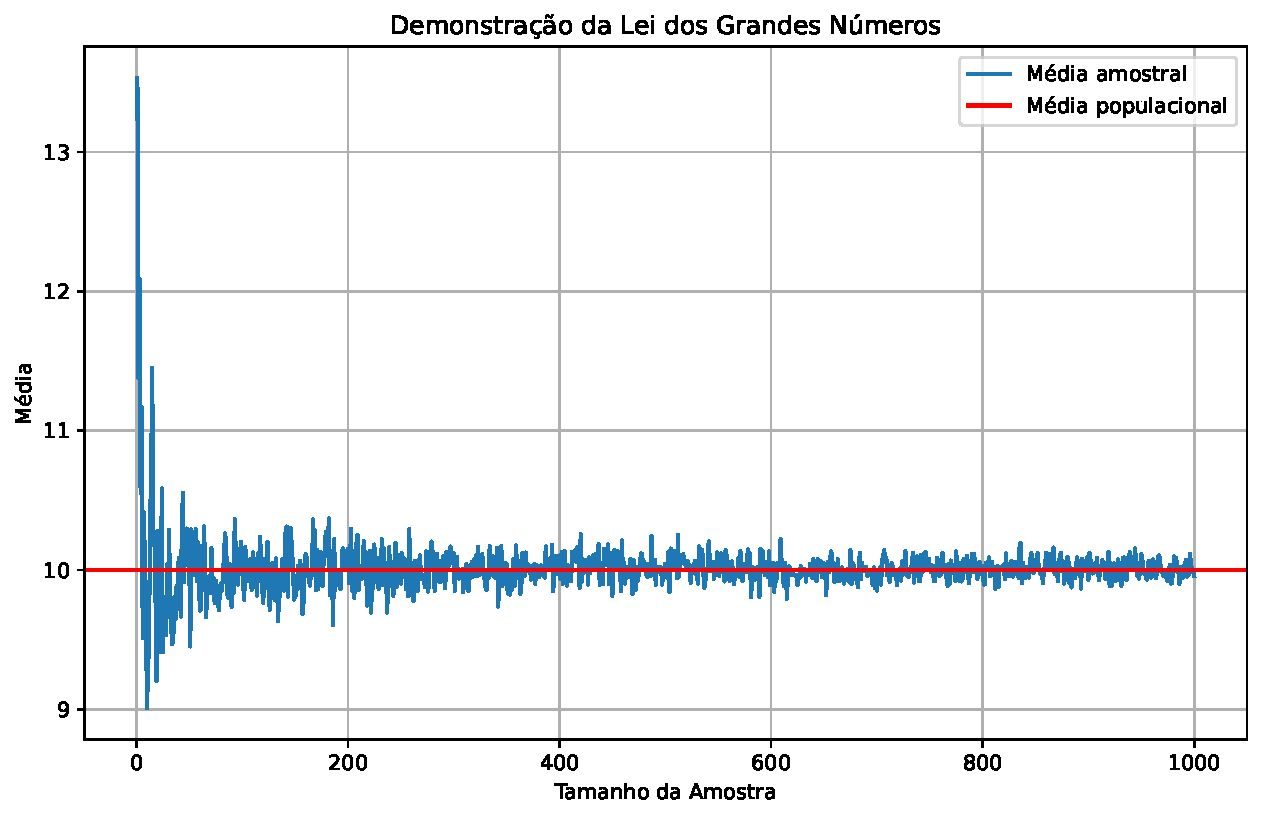
\includegraphics{intro_files/figure-pdf/cell-2-output-1.pdf}

\begin{theorem}[Teorema do Limite
Central]\protect\hypertarget{thm-limite-central}{}\label{thm-limite-central}

Sejam \(X_{1}, \ldots, X_{n}\) variáveis aleatórias independentes e
identicamente distribuídas com média \(\mu\) e variância \(\sigma^2\).
Seja \(X_n = \frac{1}{n} \sum_{i=1}^n X_i\). Então,

\[
Z_n = \frac{X_n - \mu}{\sqrt{\frac{\sigma^2}{n}}} = \frac{\sqrt{n}(X_n - \mu)}{\sigma} 
\xrightarrow[n \to \infty]{} Z
\]

onde \(Z\) tem uma distribuição normal padrão. Em outras palavras,

\[
\lim_{n \to \infty} \mathbb{P}(Z_n \leq z) = \Phi(z) = \int_{-\infty}^{z} \frac{1}{\sqrt{2 \pi}} e^{-x^2/2} \, dx.
\]

\end{theorem}

\begin{Shaded}
\begin{Highlighting}[]
\ImportTok{import}\NormalTok{ numpy }\ImportTok{as}\NormalTok{ np}
\ImportTok{import}\NormalTok{ matplotlib.pyplot }\ImportTok{as}\NormalTok{ plt}

\KeywordTok{def}\NormalTok{ tcl(N, pop):}
\NormalTok{    size\_sample }\OperatorTok{=} \DecValTok{100}
\NormalTok{    sample\_mean }\OperatorTok{=}\NormalTok{ [}
\NormalTok{        np.random.choice(pop, size}\OperatorTok{=}\NormalTok{size\_sample, replace}\OperatorTok{=}\VariableTok{True}\NormalTok{).mean() }\ControlFlowTok{for}\NormalTok{ \_ }\KeywordTok{in} \BuiltInTok{range}\NormalTok{(N)}
\NormalTok{    ]}
    \ControlFlowTok{return}\NormalTok{ np.array(sample\_mean)}

\KeywordTok{def}\NormalTok{ plot\_tcl(N\_values, pop):}

\NormalTok{    fig, axs }\OperatorTok{=}\NormalTok{ plt.subplots(}\DecValTok{1}\NormalTok{, }\BuiltInTok{len}\NormalTok{(N\_values), figsize}\OperatorTok{=}\NormalTok{(}\DecValTok{15}\NormalTok{, }\DecValTok{5}\NormalTok{), sharey}\OperatorTok{=}\VariableTok{True}\NormalTok{)}
    
    \ControlFlowTok{for}\NormalTok{ i, N }\KeywordTok{in} \BuiltInTok{enumerate}\NormalTok{(N\_values):}
\NormalTok{        sample\_means }\OperatorTok{=}\NormalTok{ tcl(N, pop)}
\NormalTok{        axs[i].hist(sample\_means, bins}\OperatorTok{=}\DecValTok{30}\NormalTok{, edgecolor}\OperatorTok{=}\StringTok{\textquotesingle{}k\textquotesingle{}}\NormalTok{, alpha}\OperatorTok{=}\FloatTok{0.7}\NormalTok{)}
\NormalTok{        axs[i].set\_title(}\SpecialStringTok{f\textquotesingle{}}\SpecialCharTok{\{}\NormalTok{N}\SpecialCharTok{\}}\SpecialStringTok{ Amostras\textquotesingle{}}\NormalTok{, fontsize}\OperatorTok{=}\DecValTok{21}\NormalTok{)}
\NormalTok{        axs[i].set\_xlabel(}\StringTok{\textquotesingle{}Média da Amostra\textquotesingle{}}\NormalTok{, fontsize}\OperatorTok{=}\DecValTok{18}\NormalTok{)}
\NormalTok{        axs[i].set\_ylabel(}\StringTok{\textquotesingle{}Frequência\textquotesingle{}}\NormalTok{, fontsize}\OperatorTok{=}\DecValTok{18}\NormalTok{)}

\NormalTok{    plt.tight\_layout(rect}\OperatorTok{=}\NormalTok{[}\DecValTok{0}\NormalTok{, }\FloatTok{0.03}\NormalTok{, }\DecValTok{1}\NormalTok{, }\FloatTok{0.95}\NormalTok{])}
\NormalTok{    plt.show()}

\NormalTok{np.random.seed(}\DecValTok{0}\NormalTok{)}
\CommentTok{\# Gerar a população}
\NormalTok{pop }\OperatorTok{=}\NormalTok{ np.random.uniform(size}\OperatorTok{=}\DecValTok{1000}\NormalTok{)}

\CommentTok{\# Plota um histograma com diferentes números de amostras}
\NormalTok{plot\_tcl([}\DecValTok{50}\NormalTok{, }\DecValTok{200}\NormalTok{, }\DecValTok{1000}\NormalTok{], pop)}
\end{Highlighting}
\end{Shaded}

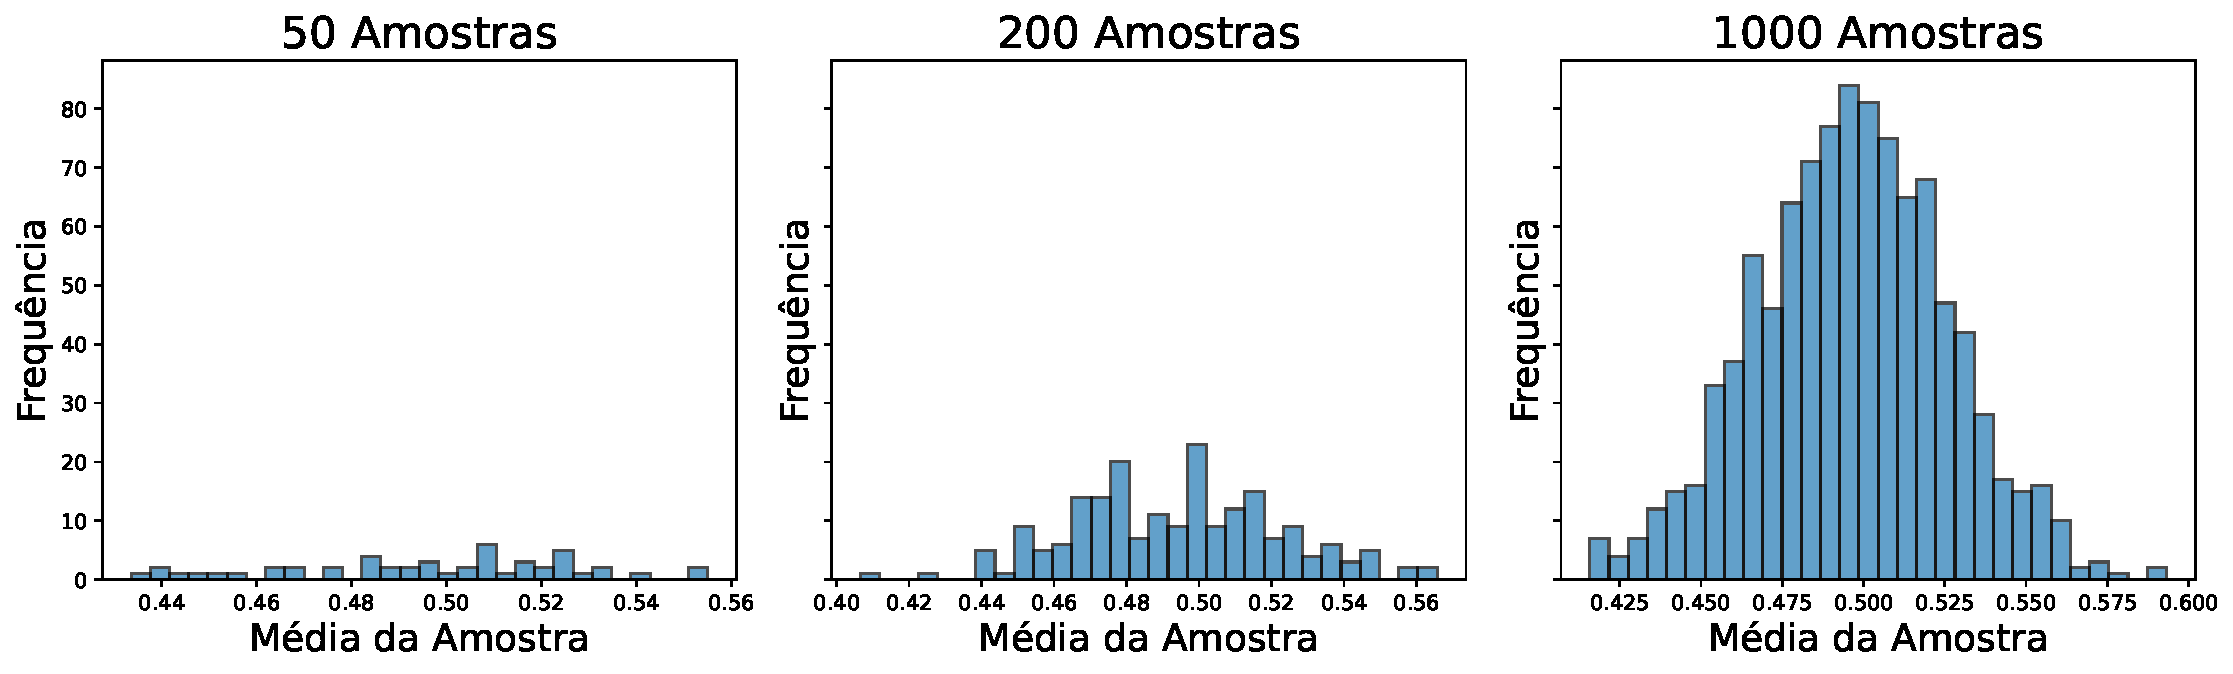
\includegraphics{intro_files/figure-pdf/cell-3-output-1.pdf}

\section{Séries de tempo}\label{suxe9ries-de-tempo}

Uma série de tempo é caracterizada por uma sequência de observações
tomada sequencialmente no tempo. Podemos chamar essa sequência de
observações \$ (y\_\{1\},y\_\{2\},y\_\{3\}\ldots) \$ como sendo
variáveis aleatórias, onde \(y = f(t) + \varepsilon_{t}\), em outras
palavras, cada observação é uma função do tempo mais um fator aleatório
(ruído branco). Como esse \(y\) depende do tempo, vamos ter um valor
diferente de \(y\) para cada valor de \(t=0,1,2,...,T\);
\(y^{*} = f(t^{*}) + \varepsilon_{t^{*}}\). Então \(y_{1}\) é o valor de
\(y\) no período 1, \(y_{2}\) é o valor de \(y\) no período 2 e assim
vai. Uma série de tempo pode ser dividida entre um processo
determinístico ou estocástico.

\subsection{Processo determinístico}\label{processo-determinuxedstico}

É um processo que não depende de um termo aleatório e sempre irá ter o
mesmo resultado dado um valor inicial. O processo \(T_{t} = 1 + 0,1t\) é
um processo determinístico, pois não depende de nenhum fator aleatório,
estando sempre acompanhado de uma constante (1) e um termo de tendência
determinística \((0,1t)\).

Podemos observar essa função melhor, gerando o seguinte gráfico no
\textbf{R}.

\subsection{Processo estocástico}\label{processo-estocuxe1stico}

O que diferencia um processo estocástico do determinístico é o fator
aleatório, por mais que esse fator seja aleatório ele apresenta uma
função de distribuição de probabilidade, por mais que se saiba qual é o
valor inicial de uma série, não dá para saber com exatidão o próximo
valor, mas podemos atribuir probabilidades a diferentes valores.

\subsubsection{Ruído Branco}\label{ruuxeddo-branco}

Um ruído branco é uma sequência serial de variáveis aleatórias não
correlacionadas com média zero e variância finita e constante, seria
aquele erro \((u)\) da primeira parte do curso. Assumimos duas condições
importantes para o ruído branco: ele deve ser independente um do outro e
deve apresentar uma distribuição normal\footnote{Chamada também de
  \emph{Distribuição normal gaussiana}.}. Sendo escrito da seguinte
forma:

\[
\begin{aligned}
\varepsilon_{t} &\sim i.i.d.\mathcal{N}(0, \sigma^2) \\
\varepsilon_{t} &\sim RB(0, \sigma^2)
\end{aligned}
\]

O ruído branco assume 3 propriedades:

\begin{itemize}
\tightlist
\item
  \(\mathbb{E}[\varepsilon_{t}] = \mathbb{E}[\varepsilon_{t} \mid \varepsilon_{t-1}, \varepsilon_{t-2}, \dotsc] = 0\)
\item
  \(\mathbb{E}[\varepsilon_{t} \varepsilon_{t-j}] = \text{cov}[\varepsilon_{t} \varepsilon_{t-j}] = 0\)
\item
  \(\text{var}[\varepsilon_{t}] = \text{cov}[\varepsilon_{t} \varepsilon_{t}] = \sigma^{2}_{\varepsilon_{t}}\)
\end{itemize}

As duas primeiras propriedades dizem respeito à impossibilidade de
preditividade e à ausência de autocorrelação. A terceira diz respeito à
homocedasticidade, a variância ser constante.

Para visualizar isso, criei uma função em \textbf{Python} que gera um
conjunto de dados de ruído branco usando a função
\emph{np.random.normal} que cria um conjunto aleatório de dados de uma
distribuição normal, onde \(n\) é o tamanho da amostra desejado.

\begin{Shaded}
\begin{Highlighting}[]
\KeywordTok{def}\NormalTok{ white\_noise(n):}
\NormalTok{    np.random.seed(}\DecValTok{0}\NormalTok{)}
\NormalTok{    white\_noise }\OperatorTok{=}\NormalTok{ np.random.normal(}\DecValTok{0}\NormalTok{, }\DecValTok{1}\NormalTok{, n)}
    
\NormalTok{    plt.clf()}
\NormalTok{    plt.plot(white\_noise)}
\NormalTok{    plt.axhline(}\DecValTok{0}\NormalTok{, color }\OperatorTok{=} \StringTok{\textquotesingle{}black\textquotesingle{}}\NormalTok{)}
\NormalTok{    plt.show()}
    
\NormalTok{white\_noise(}\DecValTok{100}\NormalTok{)}
\end{Highlighting}
\end{Shaded}

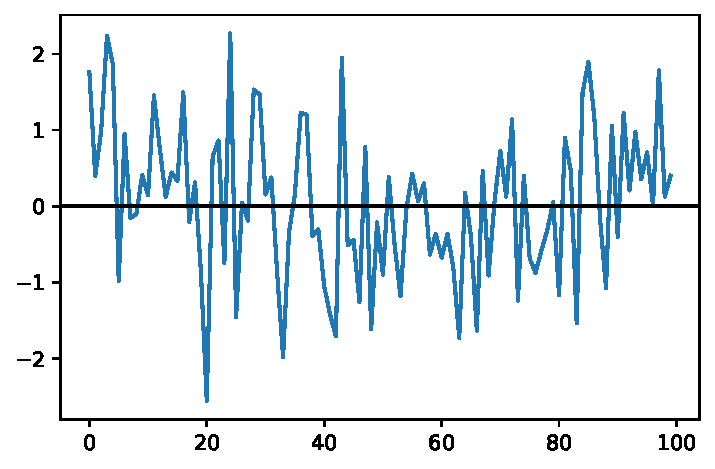
\includegraphics{intro_files/figure-pdf/cell-4-output-1.pdf}

\subsubsection{Passeio aleatório}\label{passeio-aleatuxf3rio}

Esse tempo passeio aleatório se diz pelo fato de que o valor de uma
variável em um determinado período é igual ao seu valor no período
passado mais um fator aleatório determinado por \(\varepsilon_{t}\),
sendo descrito por:

\[
y_{t} = y_{t-1} + \varepsilon_{t}
\]

Vamos supor um valor inicial para \(y_{t}\) como sendo \(y_{1}\), então:

\[
\begin{aligned}
y_{1} &= y_{0} + \varepsilon_{1} \\
y_{2} &= y_{1} + \varepsilon_{2} \\
y_{2} &= y_{0} + \varepsilon_{1} + \varepsilon_{2}
\end{aligned}
\]

Resolvendo isso recursivamente, temos:

\[
y_{t} = y_{0} + \sum_{i=1}^{t} \varepsilon_{i}
\]

Se \(y_{0} \sim 0\), podemos então dizer que o passeio aleatório é uma
soma acumulada de ruídos brancos:

\[
y_{t} = \sum_{i=1}^{t} \varepsilon_{i}
\]

Pode acontecer o caso do passeio aleatório ter uma constante \(\gamma\)
adicionada:

\[
y_{1} = \gamma + y_{0} + \varepsilon_{1}
\]

Logo, quando \(y_{0} \sim 0\), vamos ter que:

\[
y_{t} = \gamma t + \sum_{i=1}^{t} \varepsilon_{i}
\]

\begin{Shaded}
\begin{Highlighting}[]
\KeywordTok{def}\NormalTok{ random\_walk(trend, n):}
\NormalTok{    np.random.seed(}\DecValTok{0}\NormalTok{)}
    
\NormalTok{    yt }\OperatorTok{=}\NormalTok{ np.zeros(n)}
\NormalTok{    epsilon }\OperatorTok{=}\NormalTok{ np.random.normal(}\DecValTok{0}\NormalTok{,}\DecValTok{1}\NormalTok{,n)}
    \ControlFlowTok{for}\NormalTok{ t }\KeywordTok{in}\NormalTok{ np.arange(}\DecValTok{1}\NormalTok{,n):}
\NormalTok{        yt[t] }\OperatorTok{=}\NormalTok{ t }\OperatorTok{*}\NormalTok{ trend }\OperatorTok{+}\NormalTok{ np.}\BuiltInTok{sum}\NormalTok{(epsilon[:t}\OperatorTok{+}\DecValTok{1}\NormalTok{])}
    
    \ControlFlowTok{return}\NormalTok{ yt}


\KeywordTok{def}\NormalTok{ plot\_rw(trend\_list, t):}
\NormalTok{    plt.clf()}
    \ControlFlowTok{for}\NormalTok{ trend }\KeywordTok{in}\NormalTok{ trend\_list:}
\NormalTok{        rw }\OperatorTok{=}\NormalTok{ random\_walk(trend, t)}
\NormalTok{        plt.plot(rw, label}\OperatorTok{=}\SpecialStringTok{f\textquotesingle{}Tendencia = }\SpecialCharTok{\{}\NormalTok{trend}\SpecialCharTok{\}}\SpecialStringTok{\textquotesingle{}}\NormalTok{)}
    
\NormalTok{    plt.legend()}
\NormalTok{    plt.show()}

\NormalTok{trend\_list }\OperatorTok{=}\NormalTok{ [}\DecValTok{0}\NormalTok{, }\FloatTok{0.2}\NormalTok{, }\OperatorTok{{-}}\FloatTok{0.2}\NormalTok{]}
\NormalTok{plot\_rw(trend\_list, t}\OperatorTok{=}\DecValTok{100}\NormalTok{)}
\end{Highlighting}
\end{Shaded}

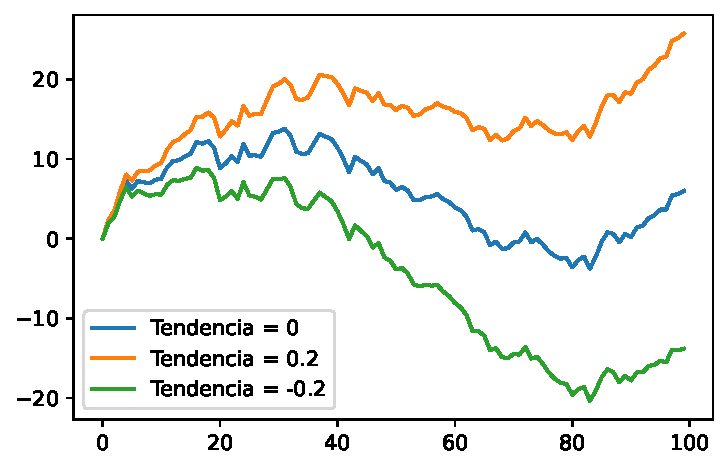
\includegraphics{intro_files/figure-pdf/cell-5-output-1.pdf}

\subsection{Estacionariedade e
Autocorrelação}\label{estacionariedade-e-autocorrelauxe7uxe3o}

Antes de entrar no assunto de autocorrelação, devemos ter em mente
algumas propriedades referentes ao primeiro momento (esperança) e
segundo momento (variância) de um passeio aleatório. O primeiro momento
de um passeio aleatório pode ser calculado pela sua média:

\[
\EX[y_{t}] = \EX[y_{0} + \sum_{i=1}^{t} \varepsilon_{i}] = \EX[y_{0}] + \EX[\sum_{i=1}^{t} \varepsilon_{i}] = \EX[y_{0}] + 0 = y_{0} = \mu
\]

Nota-se que a esperança (média) de \(y_{t}\) não depende de \(t\), sendo
uma constante e é por isso que estou chamando de \(\mu\).

O segundo momento é a variância:

\[
\text{Var}[y_{t}] = \EX[y_{t}^{2}] = \EX[(y_{t} - \EX[y_{t}])^{2}]
\] \[
= \EX[y_{t}^{2}] - \EX[y_{0}]^{2}
\] \[
= \EX[(y_{0} + \sum \varepsilon_{i})^{2}]
\] \[
= \EX[y_{0}^{2} + 2y_{0}\sum \varepsilon_{i} + \sum \varepsilon_{i}^{2}] - \mu^{2}
\] \[
= \EX[y_{0}^{2}] + 2y_{0}\sum \EX[\varepsilon_{i}] + \sum \EX[\varepsilon_{i}^{2}] - \mu^{2}
\] \[
= \mu^{2} + 0 + \sum \sigma^{2} - \mu^{2} = t \sigma^{2}
\]

Podemos observar que a variância de um processo aleatório não é
constante, pois vai depender de \(t\).

Outra parada importante é definir a covariância para \(k\) lags:

\[
\text{Cov}[y_{t},y_{t-k}] = \EX \{ (y_{t} - \EX[y_{t}])(y_{t-k} - \EX[y_{t-k}]) \} = \EX [(y_{t} - \mu)(y_{t-k} - \mu )]
\]

\subsection{Estacionariedade}\label{estacionariedade}

A hipótese da estacionariedade é um caso particular do \textbf{processo
estocástico}, no qual se assume que o processo está em um estado de
equilíbrio. O caso dos processos estritamente estacionários
(estacionariedade forte) é quando \textbf{todas} as suas propriedades
(momentos) não são afetadas pelo tempo. Como essas condições são muito
restritas, na grande maioria das vezes nos referimos a esse processo
estocástico como \textbf{fracamente estacionário}, ou
\textbf{covariância-estacionário}, ou \textbf{estacionário de segunda
ordem}. Isso quer dizer que apenas a média e a variância devem ser
constantes e que a covariância deve depender apenas do número de lags
\((k)\):

\[
\EX[y_{t}] = \mu
\] \[
\text{Var}[y_{t}] = \EX[(y_{t} - \mu)^{2}] = \sigma^2
\] \[
\text{Cov}[y_{t},y_{t+k}] = \EX [ (y_{t} - \mu)(y_{t-k} - \mu)] = \gamma_{k}
\]

\subsection{Função de autocorrelação
(FAC)}\label{funuxe7uxe3o-de-autocorrelauxe7uxe3o-fac}

Ao assumir a hipótese da estacionariedade, vamos ter que a função
conjunta de probabilidade de \(y_{t_{1}}\) e \(y_{t_{2}}\) será a mesma
para todo o tempo \(t_{1}\) e \(t_{2}\), que será constante. Isso
implica que a \textbf{covariância} entre \(y_{t}\) e \(y_{t+k}\) será
separada apenas por \(k\) intervalos de tempo (lag). Assim, a
\emph{autocovariância} ao lag \(k\) é definida por:

\[
\gamma_{k} = \text{Cov}[y_{t},y_{t+k}] = \EX [ (y_{t} - \mu)(y_{t-k} - \mu)]
\]

Da mesma forma, teremos que a \textbf{autocorrelação} é dada por:

\[
\rho_{k} = \dfrac{\EX [ (y_{t} - \mu)(y_{t-k} - \mu)]}{\sqrt{\EX[(y_{t} - \mu)^{2}] \EX[(y_{t} - \mu)^{2}] }} = \dfrac{\EX [ (y_{t} - \mu)(y_{t-k} - \mu)]}{\sigma^{2}}
\]

Como em um processo estacionário a variância é constante, vamos ter que
\(\gamma_{0} = \sigma^{2}\). Podemos então dizer que a autocorrelação no
lag \(k\) é:

\[
\rho_{k} = \dfrac{\gamma_{k}}{\gamma_{0}}
\]

E isso implica que \(\rho_{0} = 1\) se \(k=0\).

A \textbf{Função de autocorrelação} é quando se plota um gráfico
\(\rho_{k}\) contra o lag \(k\).

\bookmarksetup{startatroot}

\chapter*{Referencias}\label{referencias}
\addcontentsline{toc}{chapter}{Referencias}

\markboth{Referencias}{Referencias}

\phantomsection\label{refs}
\begin{CSLReferences}{1}{0}
\bibitem[\citeproctext]{ref-box2015time}
Box, George EP, Gwilym M Jenkins, Gregory C Reinsel, e Greta M Ljung.
2015. \emph{Time series analysis: forecasting and control}. John Wiley
\& Sons.

\bibitem[\citeproctext]{ref-enders2014applied}
Enders, W. 2014. \emph{Applied Econometric Times Series}. Wiley Series
em Probability e Statistics. Wiley.
\url{https://books.google.com.br/books?id=lmr9oQEACAAJ}.

\bibitem[\citeproctext]{ref-hamilton2020time}
Hamilton, James Douglas. 1994. \emph{Time series analysis}. Princeton
university press.

\bibitem[\citeproctext]{ref-kevinkotze}
Kotze, Kevin. 2019. {«Time Series Analusis»}. 2019.
\url{https://www.economodel.com/time-series-analysis-2019}.

\end{CSLReferences}




\end{document}
